% !TEX options=--shell-escape
\documentclass[a4paper,11pt]{scrartcl}
\usepackage[a4paper, left=2cm, right=2cm, top=2cm, bottom=3cm]{geometry}

% Umlaute in der Datei erlauben, auf deutsch umstellen
\usepackage[utf8x]{inputenc}
\usepackage[parfill]{parskip}
%\usepackage[ngerman]{babel}

% Mathesymbole und Ähnliches
%\usepackage{amsmath}
%\usepackage{mathtools}
%\usepackage{amssymb}
%\usepackage{microtype}
%\usepackage{stmaryrd}
\usepackage{logicproof}
\usepackage{verbatim}
\usepackage{sverb}
\usepackage{listings}
\usepackage{color}
\usepackage{graphicx}

\definecolor{mygreen}{rgb}{0,0.6,0}
\definecolor{mygray}{rgb}{0.5,0.5,0.5}
\definecolor{mymauve}{rgb}{0.58,0,0.82}

\lstset{ 
  backgroundcolor=\color{white},   % choose the background color; you must add \usepackage{color} or \usepackage{xcolor}; should come as last argument
  basicstyle=\footnotesize,        % the size of the fonts that are used for the code
  breakatwhitespace=true,          % sets if automatic breaks should only happen at whitespace
  breaklines=true,                 % sets automatic line breaking
  captionpos=b,                    % sets the caption-position to bottom
  commentstyle=\color{mygreen},    % comment style
  deletekeywords={...},            % if you want to delete keywords from the given language
  escapeinside={\%*}{*)},          % if you want to add LaTeX within your code
  extendedchars=true,              % lets you use non-ASCII characters; for 8-bits encodings only, does not work with UTF-8
  firstnumber=1,                   % start line enumeration with line 1000
  frame=single,                    % adds a frame around the code
  keepspaces=true,                 % keeps spaces in text, useful for keeping indentation of code (possibly needs columns=flexible)
  keywordstyle=\color{blue},       % keyword style
  language=C,                      % the language of the code
  morekeywords={*,...},            % if you want to add more keywords to the set
  numbers=left,                    % where to put the line-numbers; possible values are (none, left, right)
  numbersep=5pt,                   % how far the line-numbers are from the code
  numberstyle=\tiny\color{mygray}, % the style that is used for the line-numbers
  rulecolor=\color{black},         % if not set, the frame-color may be changed on line-breaks within not-black text (e.g. comments (green here))
  showspaces=false,                % show spaces everywhere adding particular underscores; it overrides 'showstringspaces'
  showstringspaces=false,          % underline spaces within strings only
  showtabs=false,                  % show tabs within strings adding particular underscores
  stepnumber=1,                    % the step between two line-numbers. If it's 1, each line will be numbered
  stringstyle=\color{mymauve},     % string literal style
  tabsize=2,                       % sets default tabsize to 2 spaces
  inputencoding=utf8,
  literate={å}{{\'a}}1 {ä}{{\"a}}1 {Ä}{{\"A}}1 {ö}{{\"o}}1,
  %title=\lstname                   % show the filename of files included with \lstinputlisting; also try caption instead of title
}

% Reelle, Natürliche, Ganze, Rationale Zahlen
\newcommand{\R}{\ensuremath{\mathbb{R}}}
\newcommand{\N}{\ensuremath{\mathbb{N}}}
\newcommand{\Z}{\ensuremath{\mathbb{Z}}}
\newcommand{\Q}{\ensuremath{\mathbb{Q}}}

% Fraktur für Strukturen
\newcommand{\A}{\ensuremath{\mathfrak A}}
\newcommand{\B}{\ensuremath{\mathfrak B}}
\newcommand{\C}{\ensuremath{\mathfrak C}}
\newcommand{\I}{\ensuremath{\mathfrak I}}

% Makros für logische Operatoren
\newcommand{\xor}{\ensuremath{\oplus}} %exklusives oder
\newcommand{\impl}{\ensuremath{\rightarrow}} %logische Implikation

% Meistens ist \varphi schöner als \phi, genauso bei \theta
\renewcommand{\phi}{\varphi}
\renewcommand{\theta}{\vartheta}

% Aufzählungen anpassen (alternativ: \arabic, \alph)
%\renewcommand{\labelenumi}{(\roman{enumi})}

\newcommand{\np}{
\newpage
{
    \raggedright
    \begin{tabular}{l}
        ID1206 Operating Systems \\
        Malloc \& free
    \end{tabular}}
    \hfill
    {
        \Large Seminar II
    }
    \hfill
    \begin{tabular}{r}
        Isak Nyberg\\
        \today{}
    \end{tabular}
    \hrule
}


\parskip = 0pt
\parskip = \baselineskip
\begin{document}{
\np


\section*{1. Introduction}
In the C programing language a program can use the functions free() and malloc() to allocate and deallocate data stored on the heap. This is useful for when the program needs excessively large amount of memory or dynamically needs to create data. The implementations of malloc() and free() in C uses a system call such as brk(), sbrs() or mmap() to be given a big continuous section of memory which malloc can further manipulated to give smaller sections to the program that requests it. This way a system call is not needed every time that a program needs to put data on the heap. From that point on there are many ways of implementing the ways that malloc gives data to a program, each implementation has some benefits and drawbacks.
\section*{2. Base Case}
The base case scenario of malloc creates so called blocks which consists of a head and a data section. The section data is what is returned to a program when it calls malloc. It can be manipulated by the program without consequence and is the same or greater than the size that was requested by the program. The head is the structure that will be created (or reused) every time malloc is called. It consists of 24 bytes describing relevant information that is needed for the malloc and free functions and has the following data structure:
\lstinputlisting{struct.c}
In the structure two bytes are used to determine whether the block is allocated or not, another two bytes is used to convey the size of the data part of the block. The same information about the block directly above is stored in another four bytes. Lastly each header has two sets of eight bytes that form a doubly linked list of blocks. This us only used for blocks that are free and not allocated so for an allocated block this information is redundant. This doubly linked list will be search through when a new block of a given size is needed until a fitting block is found. Thereafter if the block is big enough it will be split into two blocks, one of these will be added back to the free list and the other will be returned to the program that called malloc. This is the base case and it does provide a working system to implement malloc and free. However further optimizations can done to improve the systems performance by different metrics, this will be explored further in a later part.
\section*{2. Performance Metrics}
The system above can be evaluated in a multitude of ways. One metric that can be examined is the amount of storage that can be used. If 24 additional bytes is needed every time malloc is used suddenly a lot of space will be wasted especially if the amount requested is small. For example if malloc(8) is requested 100 times, the program will receive 800 bytes but another 2400 bytes will be used just for headers. This means in effect only 33\% of the data is actually useful to the program that called malloc. This scenario is of course an outlier and it is not very likely a program will allocate a large number of small structures on the heap. However the efficiency of the memory used can be a good metric to measure how well the malloc and free systems are functioning.\\
Another benchmark is the so called fragmentation in memory after some time of using malloc and free. If there are many blocks of a small size that are free then a malloc request for a size that is smaller than the total amount of free space might still not fit anywhere because there is no single block that is large enough to hold the entire requested size. This metric is correlated with the number of free blocks and ideally the fewer free blocks for a given amount of free size the better.
\section*{3. Benchmark}
\lstinputlisting{benchmark_psudo.c}
This is the benchmark that will be used to simulate the real usage of malloc and free (for the sake of conciseness many parts of the code is not included). It will be tested for different number of total blocks in use and different metrics can be recorded after the benchmark has terminated. The benchmark will go through 1000 iterations of freeing and allocating a random block in memory of a random size. This way the benchmark will simulate a realistic scenario as closely as possible.
\section*{4. Improvements}
\subsection*{4.1. Merging free blocks}
In the base implementation of free, the freed block is simply added to the doubly linked list of other free blocks without any other consideration. However an improvement to this process can be made in order to reduce fragmentation. In addition to before, a block should also check if the block above or a block below in the heap space is also free. If that is the case instead of appending a new block to the free list the freed block should instead merge with the existing block that is either above or below. This will cause the number of blocks in the free list to be smaller compared to before and thus fragmentation of free memory will be reduced. 
\newpage
\begin{figure}[htp]
    \centering
    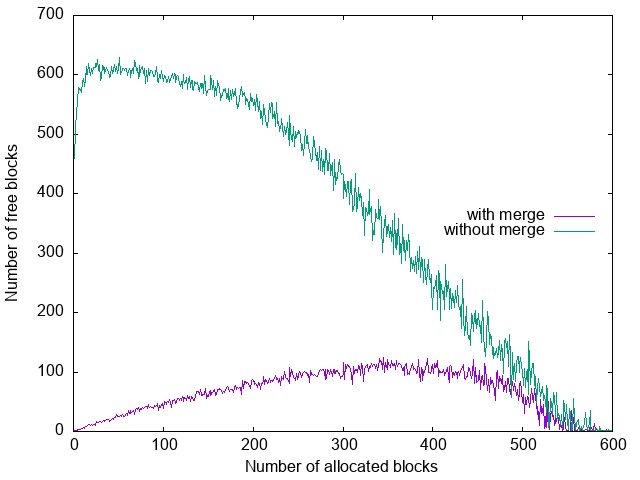
\includegraphics[width=10cm]{gnuplot/fragmentation.png}
    \caption{Fragmentation with and without merge strategy.}
    \label{fig:Graph}
\end{figure}
In figure 1 is the comparison of the length of the free list as different number of blocks is allocated. The number of blocks is capped at 600 since that is the point at which the heap if full. It is clear that when using the merge strategy the length of the free list decreases drastically. especially for a small number of allocated blocks. This improves the malloc and free system is multiple ways. Firstly it faster to find space for new blocks since the list of free blocks is shorter overall and secondly the chance of a block being able to fit is also larger since the average size of the free blocks is larger. Thus overall this is a good improvement to the free function.
\subsection*{4.2. Multiple free lists}
Another possible improvement is to reduce the computation needed to find a suitable block for currently there is a single unordered list that has all of the free blocks in it. This means that when a large malloc call is made it may need to search through multiple smaller blocks before it finds a block of the correct size. This can be improved in a few ways, the list could perhaps be sorted and then a binary search would have no problems finding blocks of suitable size efficiently. However another way would be to simple divide the single list into multiple other lists for blocks of different sizes.
\lstinputlisting{free_lists.c}
In the code above, 4 lists have been implemented to deal with blocks of different block sizes, namely for blocks in the range 0 to 64 bytes, 65 to 256 bytes, 257 to 512 bytes and blocks bigger than 512. These sizes were chosen rather arbitrarily and the number of lists and the range of each can be tailored to fit different scenarios, but for now the performance will be compared for this configuration versus the base case. (Both scenarios also include block merging when blocks are freed).
\newpage
\begin{figure}[htp]
    \centering
    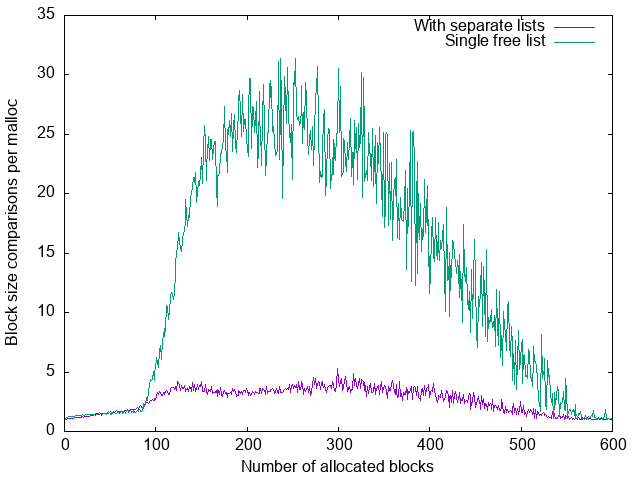
\includegraphics[width=10cm]{gnuplot/find_call.png}
    \caption{Performance of the malloc function.}
    \label{fig:Graph}
\end{figure}
This time a counter was kept that kept track on how many times a block was successfully allocated and another counter how many times a block size comparison was done and then the latter was divided by the former to find the average number of block size comparisons for each successful malloc. In figure 2 it is very apparent that when multiple lists is used the amount of computation needed to find a suitable block is drastically reduced. From this it can already be concluded that the usage of multiple lists is clearly an improvement over a single list. The number of lists and the range of sizes for each lists is something that can be optimized further. 
\section*{5. Evaluation}
Both the usage of merge when freeing blocks and the use of multiple free lists improved different metrics for the malloc and free functions. The extent to which they did is also quite drastic which means that these are very useful improvements. The way that multiple lists is implemented can be further explored since there are multiple factors that determine how much it improved performance such as the number of lists and the range of sizes in them. 
\section*{6. Conclusion}
The two different improvements explored showed significance increases in performance metric. In particular the computation needed to find blocks and the length of the free list after some time of allocating and freeing random amounts of data as simulated by a benchmark program. Further possible optimizations include reducing the size of the header to increase the amount of effectively allocated memory. This could be done through combining the free and bfree flags into the first bit of the size and bsize tag in the header (since the size is a multiple of 8 the first 3 bits are always 0). The prev and next pointers could also point to an address relative to the first block and thus only need to be 2 bytes instead of 8. Both of these optimizations combined would bring the total header from 24 bytes down to 8 bytes. Also the next and prev pointers are not needed once a block is allocated which means that those bytes can be used by the program instead of the header. In addition the usage of multiple arenas combined with multiple threads can be explored further. 
\end{document}
